\documentclass[11pt]{article}
\usepackage[final]{acl}
\usepackage{times}
\usepackage{latexsym}
\usepackage{fontspec}
\usepackage{polyglossia}
\setdefaultlanguage{russian}
\setotherlanguage{english}
\setmainfont{Times New Roman}
\newfontfamily\cyrillicfont{Times New Roman}
\usepackage{microtype}
\usepackage{inconsolata}
\usepackage{graphicx}

\title{Анализ текстовой коллекции и базовые методы обработки текста}

\author{Игорь Пивнев, ИТМО}

\begin{document}
\maketitle

\begin{abstract}
В работе проводится базовый анализ текстовой коллекции WikIR (подмножество en1k),
включая вычисление статистик, построение частотных распределений, а также проверку
эмпирических законов Ципфа и Хипса. Дополнительно рассматриваются биграммы и
методы морфологической нормализации (стемминг, лемматизация, BERT-токенизация).
В расширенной части проводится сравнение словарей художественных текстов и анализ
различий между текстами, написанными людьми и сгенерированными моделями.
\end{abstract}

\section{Постановка задачи}

Целью работы является изучение свойств текстовой коллекции и применение базовых
методов обработки естественного языка. В рамках задания необходимо:

\begin{itemize}
    \item вычислить основные статистики коллекции;
    \item построить частотный словарь слов и биграмм;
    \item проанализировать распределения (законы Ципфа и Хипса);
    \item применить методы морфологической обработки;
    \item исследовать дополнительные задачи (анализ авторских словарей и детекция
    сгенерированных текстов).
\end{itemize}

\section{Описание данных}

Основной датасет — коллекция WikIR (подмножество en1k), представляющая собой набор
текстовых документов, уже очищенных, токенизированных и приведенных к нижнему регистру.

Для анализа использовались:
\begin{itemize}
    \item $\sim$ \textbf{369721} документов;
    \item тексты на английском языке;
    \item список стоп-слов (стандартный список NLTK).
\end{itemize}

Дополнительно использовались:
\begin{itemize}
    \item тексты Л.Н. Толстого (\textit{Война и мир});
    \item тексты Ф.М. Достоевского (\textit{Братья Карамазовы});
    \item датасет CoAT для анализа сгенерированных текстов.
\end{itemize}

\section{Методы и инструменты}

Для анализа применялись следующие инструменты:
\begin{itemize}
    \item \textbf{Python} (pandas, collections, numpy);
    \item \textbf{matplotlib} для визуализации;
    \item \textbf{NLTK} (Porter Stemmer) для стемминга;
    \item \textbf{spaCy} для лемматизации;
    \item \textbf{transformers} (BERT tokenizer) для субсловной токенизации.
\end{itemize}

Частотный словарь строился с использованием структуры \texttt{Counter}. Для
биграмм использовались последовательные пары слов внутри документов.

Для анализа распределений:
\begin{itemize}
    \item закон Ципфа — зависимость частоты слова от его ранга;
    \item закон Хипса — зависимость размера словаря от числа обработанных слов.
\end{itemize}

\section{Результаты и интерпретация}

\subsection{Базовые статистики}

Были получены следующие характеристики коллекции:

\begin{itemize}
    \item количество документов: \textbf{369721};
    \item общее число слов: \textbf{73093729};
    \item средняя длина документа: \textbf{197.70};
    \item число уникальных слов: \textbf{794568};
    \item средняя длина слова: \textbf{4.80};
\end{itemize}

Полученные значения соответствуют ожидаемым для текстовых коллекций: наблюдается
большое количество редких слов и умеренная средняя длина документа.

\subsection{Частотный анализ}

Частотный словарь показывает, что наиболее частотные слова в основном являются
стоп-словами (например, \textit{the, of, and}). Общее число вхождений стоп-слов
составляет \textbf{29387785}.

При этом не все слова из топ-30 входят в стандартный стоп-лист, что указывает на
возможность его расширения в зависимости от задачи.

\subsection{Закон Ципфа}

На Рис.~\ref{fig:zipf} представлен график зависимости частоты слова от ранга в
логарифмических координатах.

\begin{figure}[h]
    \centering
    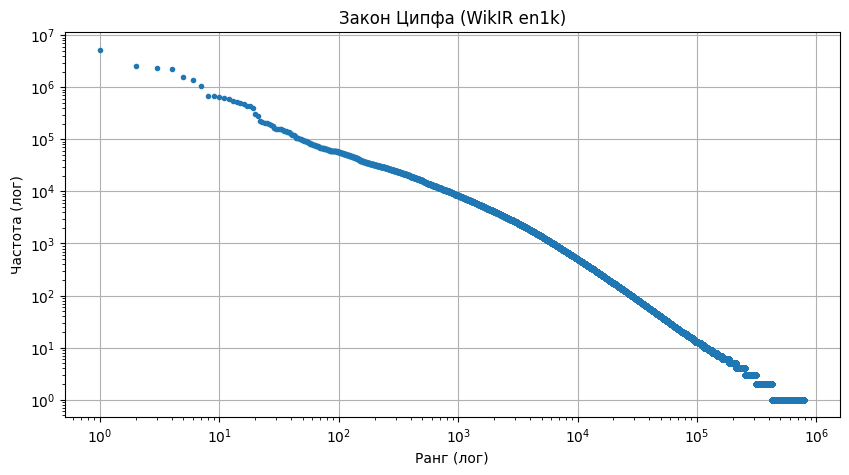
\includegraphics[width=\columnwidth]{zipf.png}
    \caption{Закон Ципфа для коллекции WikIR}
    \label{fig:zipf}
\end{figure}

Наблюдается близкое к линейному поведение в лог-лог масштабе, что подтверждает
выполнение закона Ципфа: частота слова обратно пропорциональна его рангу.

\subsection{Закон Хипса}

На Рис.~\ref{fig:heaps} показан рост словаря по мере обработки текста.

\begin{figure}[h]
    \centering
    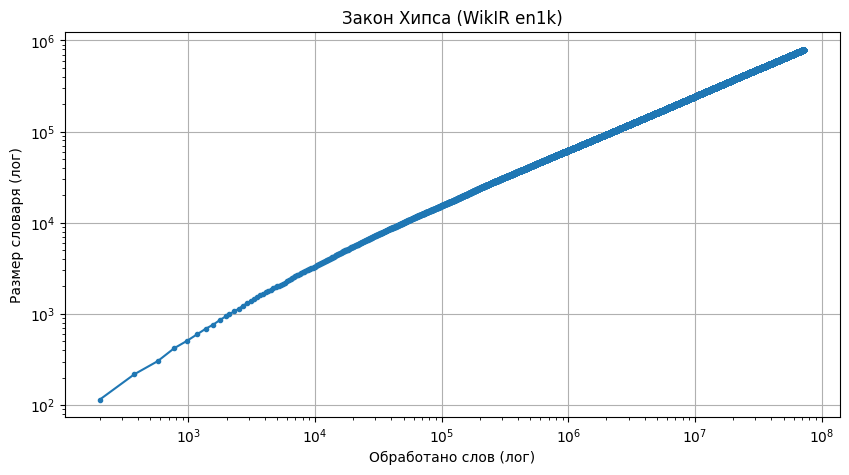
\includegraphics[width=\columnwidth]{heaps.png}
    \caption{Закон Хипса для коллекции WikIR}
    \label{fig:heaps}
\end{figure}

Зависимость имеет степенной характер, что соответствует закону Хипса: словарь
растет сублинейно относительно числа токенов.

\subsection{Биграммы}

Количество уникальных биграмм составило \textbf{12993004}. В топе частотного списка
преобладают комбинации стоп-слов (например, \textit{of the}).

Такие биграммы несут мало семантической информации, поэтому при построении словаря
для поисковых систем целесообразно использовать дополнительные критерии отбора
(например, исключение стоп-слов или использование метрик ассоциации).

\subsection{Морфологическая обработка}

Сравнение различных методов токенизации показало:

\begin{itemize}
    \item стемминг уменьшает размер словаря за счет агрессивного усечения слов;
    \item лемматизация сохраняет более корректные словоформы;
    \item BERT-токенизация увеличивает число токенов за счет разбиения на подслова.
\end{itemize}

Численные результаты:

\begin{itemize}
    \item оригинал: \textbf{988313} токенов, \textbf{61757} уникальных;
    \item стемминг: \textbf{988313} токенов, \textbf{48506} уникальных;
    \item лемматизация: \textbf{988472} токенов, \textbf{54275} уникальных;
    \item BERT: \textbf{1098605} токенов, \textbf{25702} уникальных;
\end{itemize}

\section{Анализ и обсуждение}

Полученные результаты соответствуют классическим свойствам текстовых данных:

\begin{itemize}
    \item распределение слов подчиняется закону Ципфа;
    \item рост словаря описывается законом Хипса;
    \item значительная доля частотного распределения приходится на стоп-слова.
\end{itemize}

\textbf{Ограничения и возможные улучшения:}

\begin{itemize}
    \item использование простого списка стоп-слов может быть недостаточным — его
    можно адаптировать под конкретную коллекцию;
    \item для биграмм стоит применять более продвинутые меры (например, PMI);
    \item анализ проводился без учета семантики (например, через эмбеддинги);
    \item для детекции сгенерированных текстов можно использовать более сложные
    признаки (перплексия, языковые модели).
\end{itemize}

В целом, проведенный анализ демонстрирует базовые закономерности текстовых
коллекций и может служить основой для построения поисковых и NLP-систем.

\end{document}
